\documentclass[12pt,letterpaper]{scrartcl}
\usepackage{lipsum}
\usepackage[utf8]{inputenc}
\usepackage{amsmath}
\usepackage{amsfonts}
\usepackage{amssymb}
\usepackage{graphicx}
\usepackage[left=3cm,right=2.5cm,top=2.5cm,bottom=2.5cm]{geometry}
\usepackage[]{algorithm2e}
\author{Don cuyi}

%Color
\usepackage{color}
\definecolor{nred}{RGB}{174,49,54}
\definecolor{nblue}{RGB}{86,99,146}
\definecolor{nalgo}{RGB}{188,139,76}
\usepackage{sectsty}
\sectionfont{\color{nred}}
\subsectionfont{\color{nblue}}
\subsubsectionfont{\color{nalgo}}

%Librías tikz
\usepackage{pgf,tikz}
\usepackage{mathrsfs}
\usetikzlibrary{arrows}
\usetikzlibrary[patterns]
\newcommand{\degre}{\ensuremath{^\circ}}
\definecolor{qqwuqq}{rgb}{0.,0.39215686274509803,0.}
\definecolor{ffttww}{rgb}{1.,0.2,0.4}
%Hipervinculos
\usepackage{hyperref}

\usepackage{fancyhdr}
\pagestyle{fancy}
\fancyhead[L]{Combinatoria}
\fancyhead[C]{Licenciatura en ciencias de la computación}
\fancyhead[R]{USACH}

%interlineado
\renewcommand{\baselinestretch}{1.2}

%\bibitem{Yahoo} \textsc{Andres G} (2009),
%\textbf{¿Generar números aleatorios negativos en Lenguaje C?} En \textsc{Yahoo! respuestas}
%Recuperado el el 23 del julio del 2014
%\url{https://es.answers.yahoo.com/question/index?qid=20091121055249AAUQH3N}

\newcommand{\biblio}[7]{
\bibitem{#1} \textsc{#2} (#3),
\textbf{#4} En \textsc{#5}
Recuperado el #6
\url{#7}
}

% Last, F. M. (Year Published) Book. City, State: Publisher.
\newcommand{\book}[5]{
\bibitem{#1} \textsc{#2} (#3),
\textbf{#4}  \textsc{#5} Estado: Publicado
}

\begin{document}

\begin{titlepage}

\begin{center}

{\Large { Licenciatura en ciencia de la computación} }


\includegraphics[scale=1]{UDSCNRJ}
\\[1cm]

{\Huge \textsc{Algoritmo Euclideano}}\\[0.7cm]

{\huge  Matemática Computacional}\\[2cm]


\begin{minipage}[l]{0.4\textwidth}
	\begin{flushleft}
	\linespread{1}
		\textbf{\textsf{Profesor:}}\\
		\large Nicolas Thériault
	\end{flushleft}
\end{minipage}
\begin{minipage}[l]{0.4\textwidth}

	\begin{flushright}

		\textbf{\textsf{Autor:}}\\
		\linespread{1}
		\large Sergio Salinas\\
		\large Danilo Abellá\\

	\end{flushright}
\end{minipage}

\end{center}

\end{titlepage}



\newpage
\section*{Introducción}

Informe sobre las diferentes implentaciones del Algoritmo Euclidiano.

En la implemetanción se uso la librería GNU MP 6.1.1 en C++.

Para crear los gráficos se crearon dos números al azar a y b, además al número a se le sumo el número $2^n$, donde n es la cantidad de bits a calcular, de esta forma, a siempre cumplia con la contidad de bits que se pedia.

Los gráficos fueron creado usando un script en R.


\section{Algoritmo Implementado}

A continuación se mostrará que tan eficientes fueron los distintos tipos de algoritmos.

\subsection{Algoritmo Euclidiano Simple}

Este algoritmo demostró ser altamente ineficiente dado que cuando se trabaja con números muy grandes el tiempo requerido es muy alto, a pesar de que su lógica sea muy simple.
Tiempos de espera para los siguientes gcd:
\\\\
gcd(291,252) - 0.0002230 segundos
\\
gcd(16261,85652) - 0.0002450 segundos
\\
gcd(897279761,914407221) - 0.0009650 segundos
\\
gcd(16534528044,8332745927) - 0.0008580 segundos
\\
gcd(43263441545690516,43312793054108111) - 0.0068580 segundos


\subsection{Algoritmo Euclidiano}

Este algoritmo resultó ser la mejor opción en cuanto a complejidad y eficiencia ya que no demostró una lógica muy complicada ni un tiempo de espera demasiado alto, aunque no halla sido de los que menos tiempo de ejecución requirió.
\\
Tiempos de espera para los siguientes gcd:
\\\\
gcd(291,252) - 0.0000610 segundos
\\
gcd(16261,85652) - 0.0000780 segundos
\\
gcd(897279761,914407221) - 0.0000780 segundos
\\
gcd(16534528044,8332745927) - 0.0000920 segundos
\\
gcd(43263441545690516,43312793054108111) - 0.0000960 segundos
\\
gcd(23356764234689876532233456788876543234567,\\
6277101735386680763835789423207666416083908700390324961279) - 0.0001140 segundos
\\
gcd(2123010620889223608977186369097185643295866022\\04480027488784019561937182491149755503041950,\\
68185362149486650485123987197513787717187652289362\\47143232679847194284772046122091468887714) - 0.0002170 segundos


\newpage

\subsection{Algoritmo Euclidiano Binario}

Este algoritmo estubo de entre los más eficientes ya que a pesar de su complejidad fue uno de los más rápidos en ejecutarse.
\\
Tiempos de espera para los siguientes gcd:
\\\\
gcd(291,252) - 0.0000510 segundos
\\
gcd(16261,85652) - 0.0000580 segundos
\\
gcd(897279761,914407221) - 0.0000630 segundos
\\
gcd(16534528044,8332745927) - 0.0000610 segundos
\\
gcd(43263441545690516,43312793054108111) - 0.0000780 segundos
\\
gcd(23356764234689876532233456788876543234567,\\
6277101735386680763835789423207666416083908700390324961279) - 0.0000730 segundos
\\
gcd(2123010620889223608977186369097185643295866022\\04480027488784019561937182491149755503041950,\\
68185362149486650485123987197513787717187652289362\\47143232679847194284772046122091468887714) - 0.0001170 segundos

\subsection{Algoritmo Euclidiano Extendido}

Este sin duda resultó ser el algoritmo con tiempo de espera más corto haciendolo el más eficiente de todos los evaluados anteriormente.
Tiempos de espera para los siguientes gcd:
\\\\
gcd(291,252) - 0.0000350 segundos
\\
gcd(16261,85652) - 0.0000340 segundos
\\
gcd(897279761,914407221) - 0.0000360 segundos
\\
gcd(16534528044,8332745927) - 0.0000400 segundos
\\
gcd(43263441545690516,43312793054108111) - 0.0000410 segundos
\\
gcd(23356764234689876532233456788876543234567,\\
6277101735386680763835789423207666416083908700390324961279) - 0.0000700 segundos
\\
gcd(2123010620889223608977186369097185643295866022\\04480027488784019561937182491149755503041950,\\
68185362149486650485123987197513787717187652289362\\47143232679847194284772046122091468887714) - 0.0001410 segundos

\newpage
\subsection{Algoritmo Euclidiano Extendido Binario}

Pese que con números de pocas unidades el programa tiene un tiempo de ejecución a la par con el resto de algoritmos, cuando se utilizan números con muchas cifras ( > 10 ) ya el tiempo de espera se dispara quedando bastante atrás con respecto a sus otras opciones.
Tiempos de espera para los siguientes gcd:
\\\\
gcd(291,252) - 0.0000390 segundos
\\
gcd(16261,85652) - 0.0000420 segundos
\\
gcd(897279761,914407221) - 0.0000570 segundos
\\
gcd(16534528044,8332745927) - 0.0000620 segundos
\\
gcd(43263441545690516,43312793054108111) - 0.0000910 segundos
\\
gcd(23356764234689876532233456788876543234567,\\
6277101735386680763835789423207666416083908700390324961279) - 0.0002210 segundos
\\
gcd(2123010620889223608977186369097185643295866022\\04480027488784019561937182491149755503041950,\\
68185362149486650485123987197513787717187652289362\\47143232679847194284772046122091468887714) - 0.0004830 segundos

\newpage
\section{Formulación experimentos}

\section{Información de Hardware y Software}


\subsection{ Notebook - Danilo Abellá}
\subsubsection{Software}
\begin{itemize}
\item SO: Xubuntu 16.04.1 LTS
\item GMP Library
\item Mousepad 0.4.0
\end{itemize}

\subsubsection{Hardware}
\begin{itemize}
\item AMD Turion(tm) X2 Dual-Core Mobile RM-72 2.10GHz
\item Memoria (RAM): 4,00 GB(3,75 GB utilizable)
\item Adaptador de pantalla: ATI Raedon HD 3200 Graphics
\end{itemize}



\subsection{Notebook - Sergio Salinas}
\subsubsection{Software}
\begin{itemize}
\item  SO: ubuntu Gnome 16.04 LTS
\item Compilador: gcc version 5.4.0 20160609 
\item Editor de text: Atom
\end{itemize}

\subsubsection{Hardware}
\begin{itemize}
\item Procesador: Intel Core i7-6500U CPU  2.50GHz x 4 
\item Video: Intel HD Graphics 520 (Skylake GT2) 
\end{itemize}


\newpage

\section{Curvas de desempeño de resultados}

\subsection{Algoritmo 2}

\begin{center}
	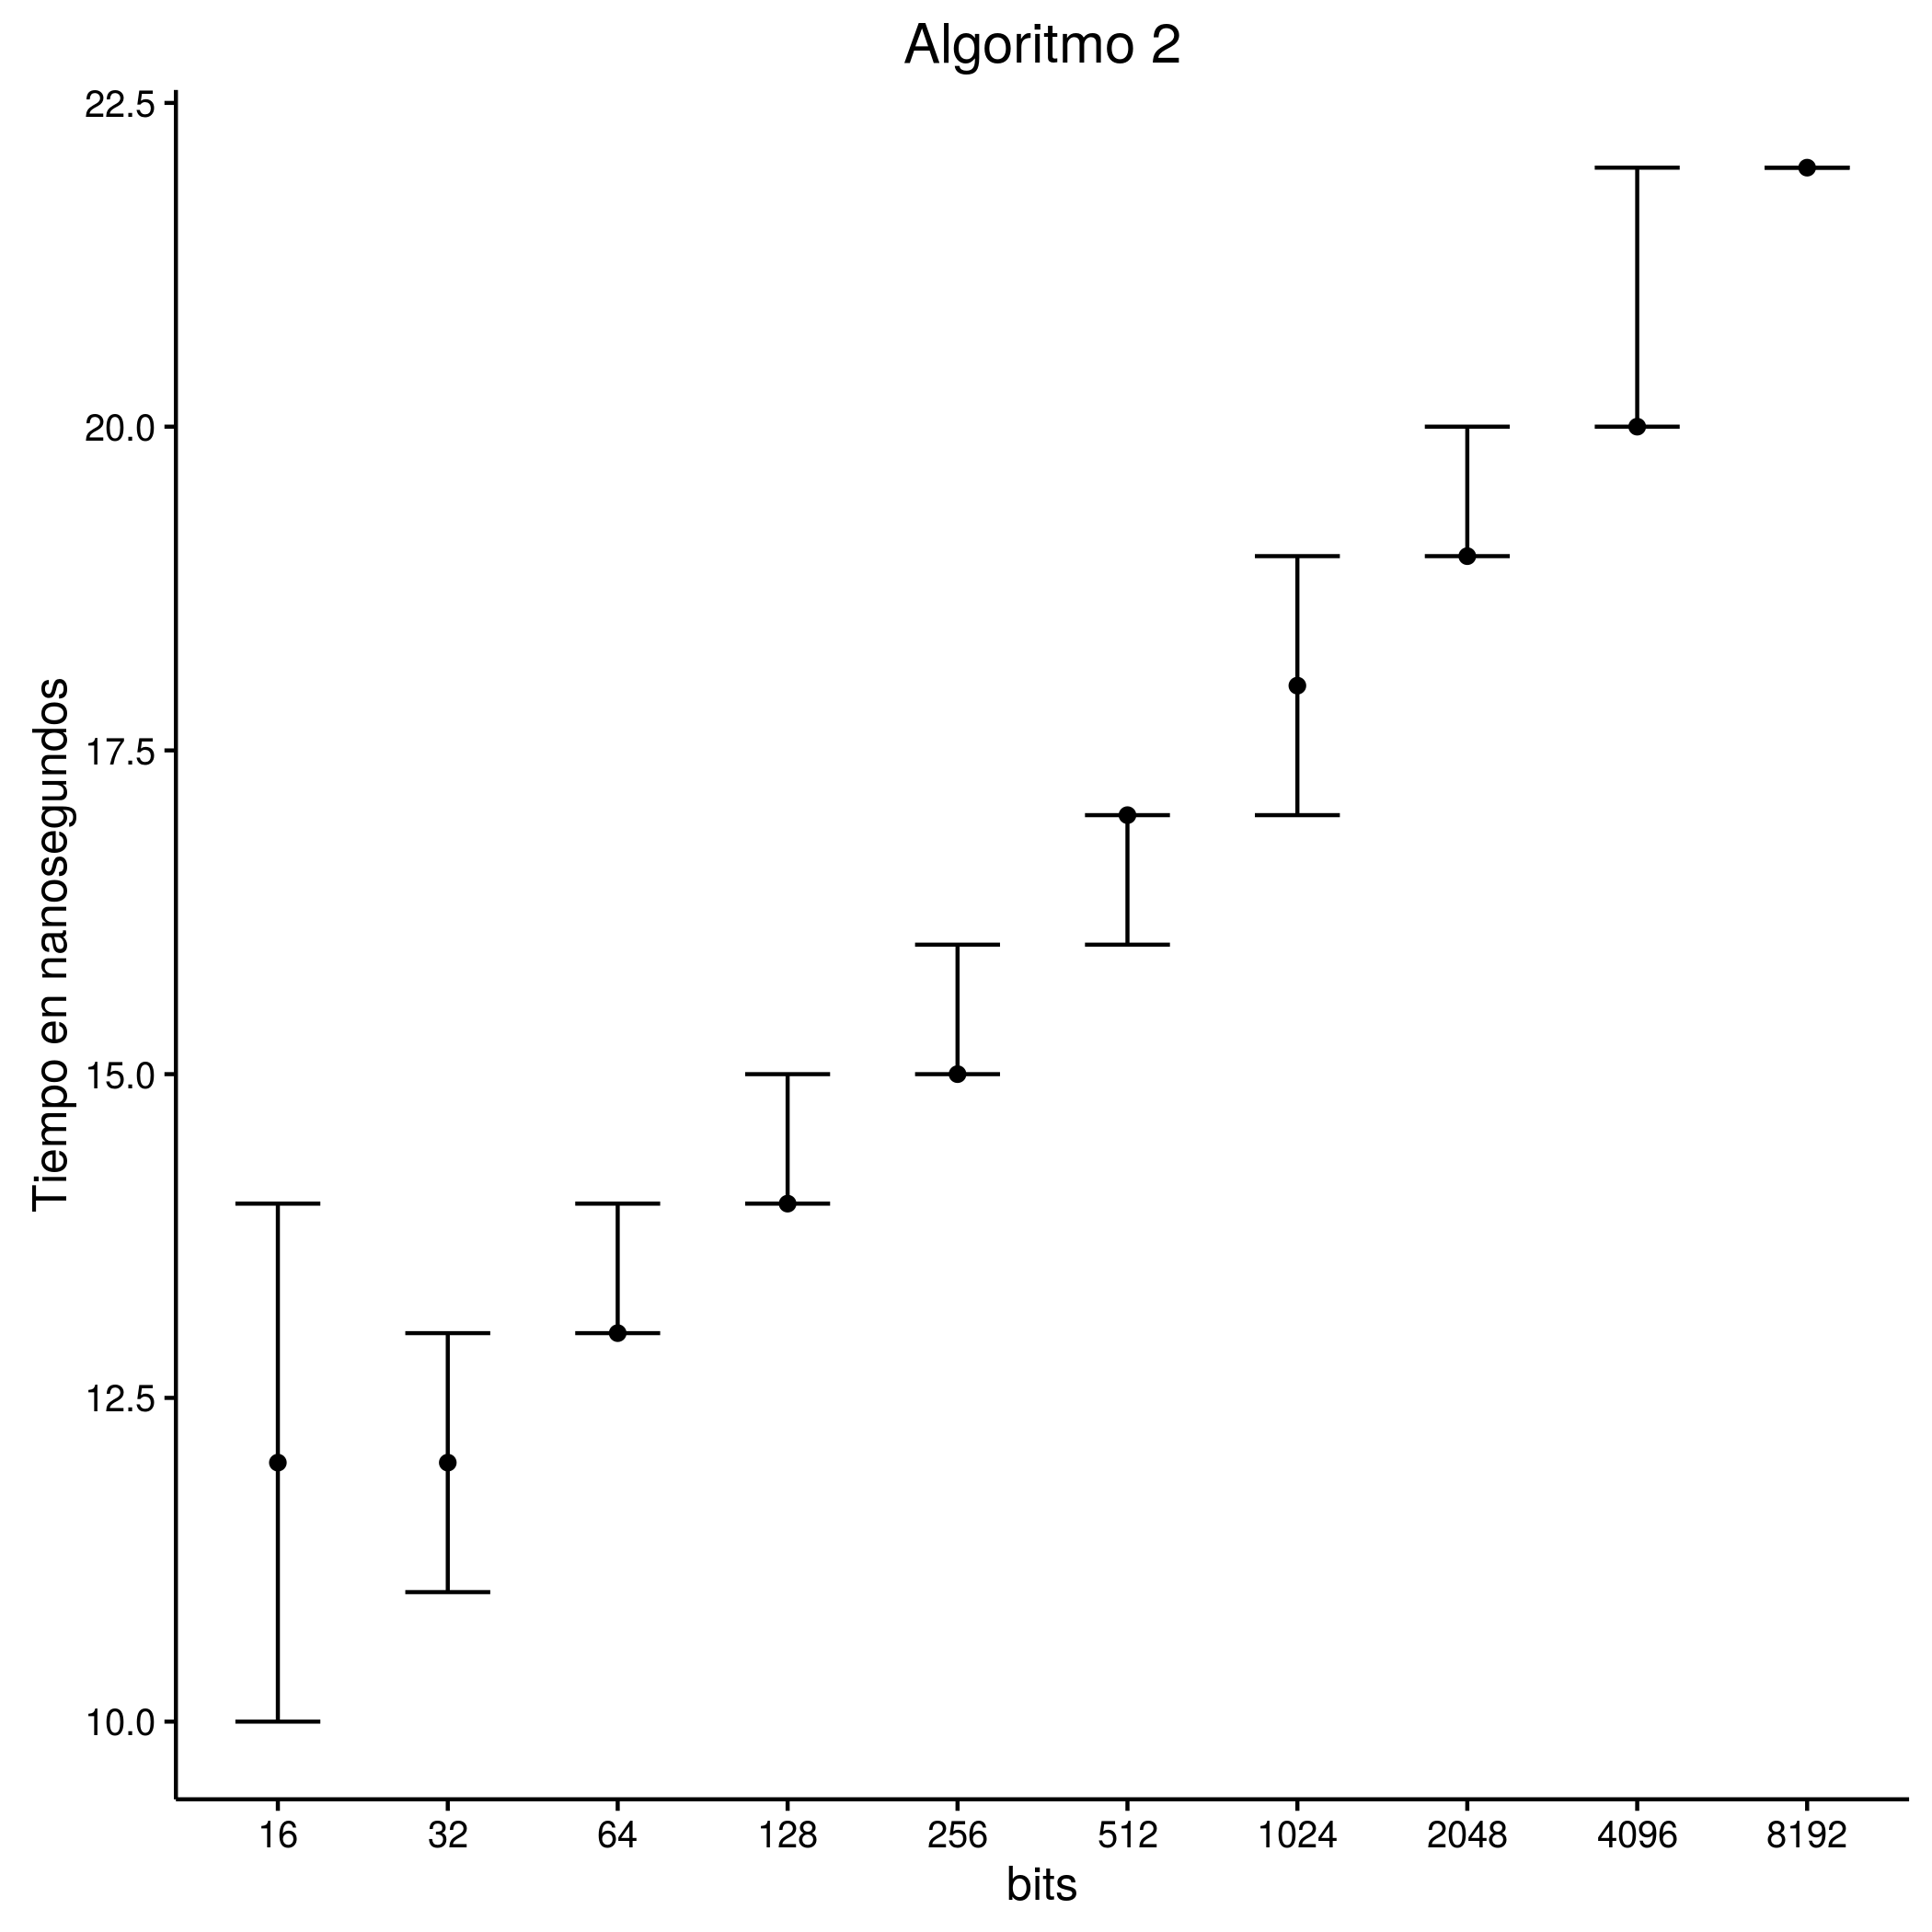
\includegraphics[scale=1]{plot/a2.png}
\end{center}	

\newpage


\subsection{Algoritmo 3}

\begin{center}
	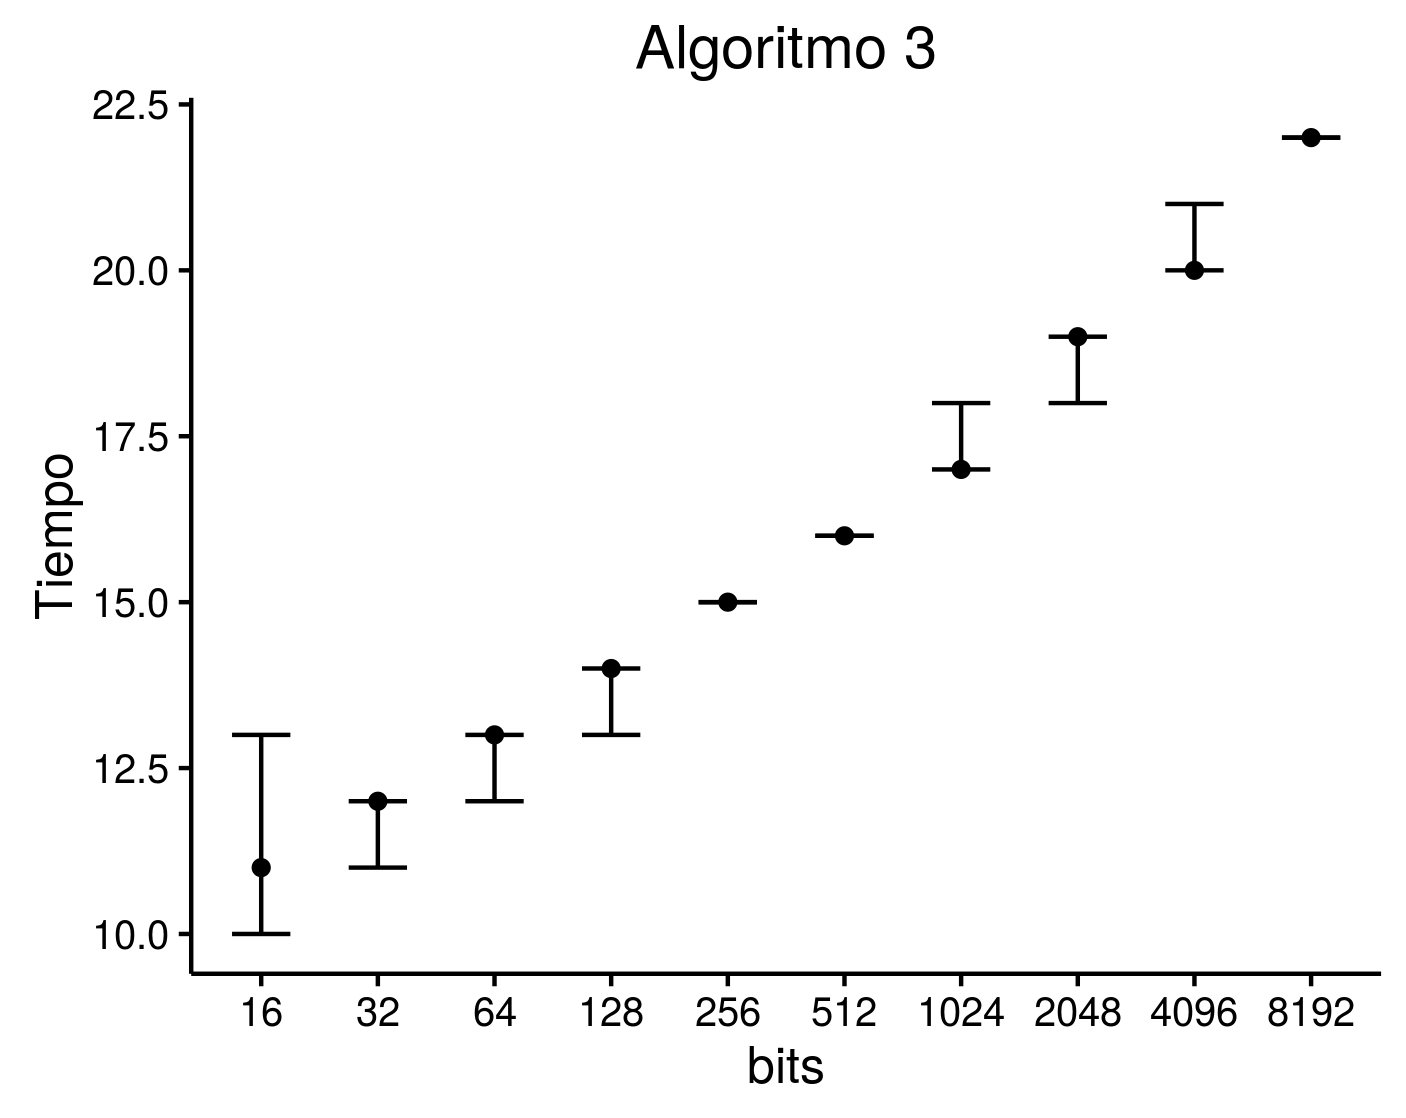
\includegraphics[scale=1]{plot/a3.png}
\end{center}	

\newpage


\subsection{Algoritmo 4}

\begin{center}
	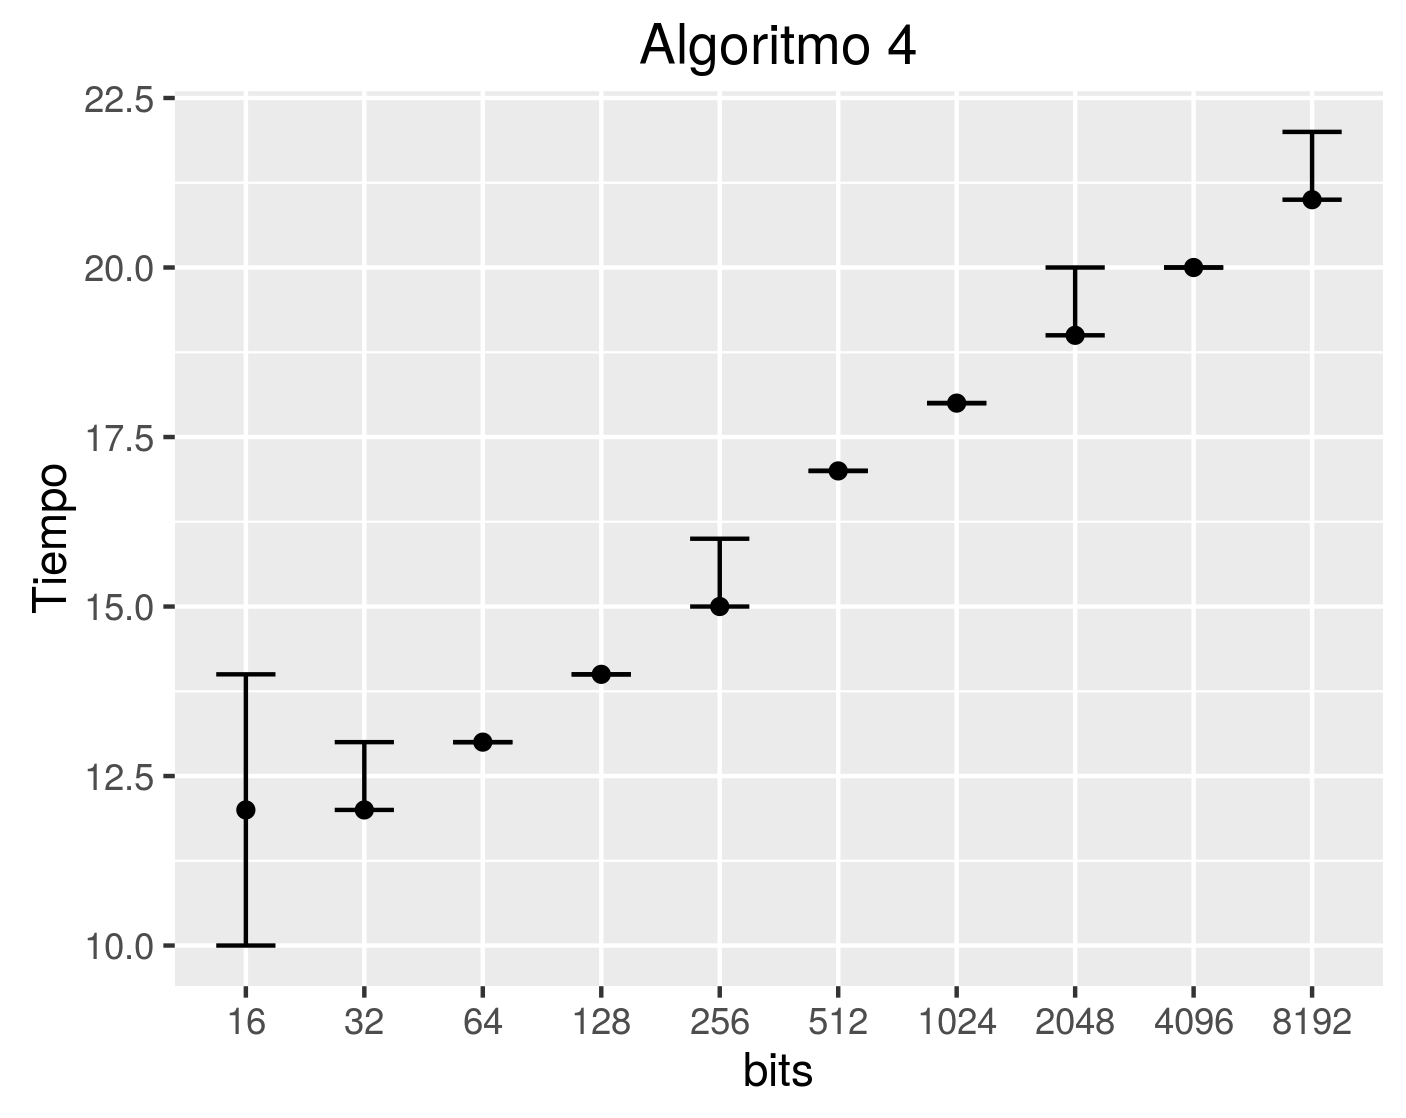
\includegraphics[scale=1]{plot/a4.png}
\end{center}	

\newpage


\subsection{Algoritmo 5}

\begin{center}
	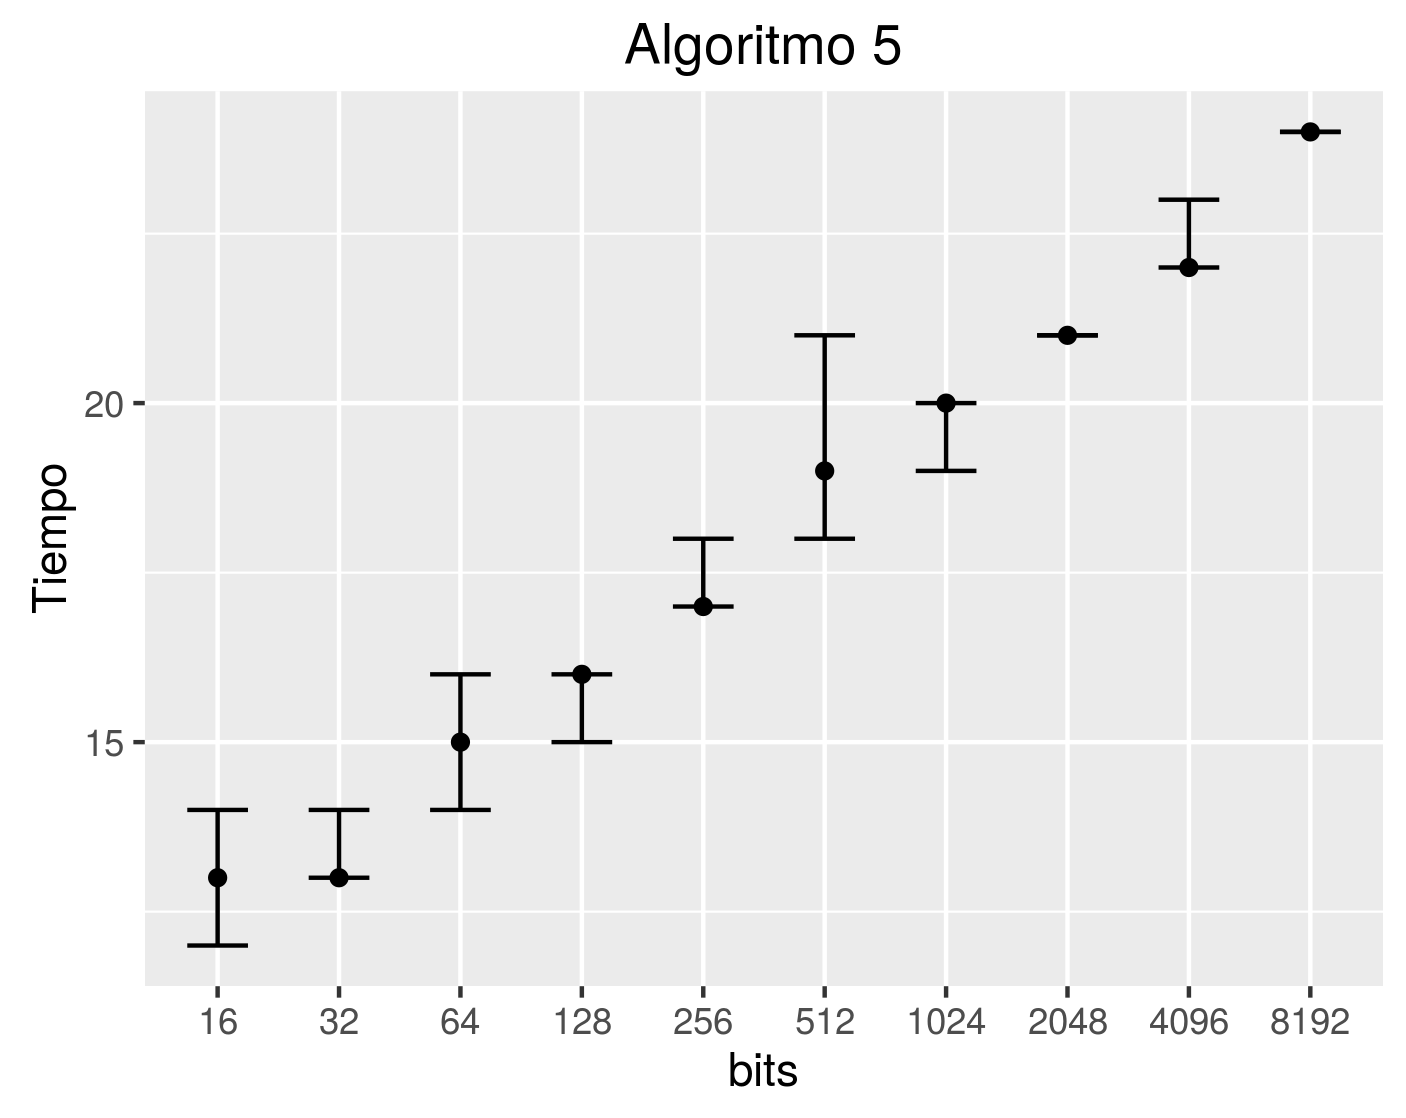
\includegraphics[scale=1]{plot/a5.png}
\end{center}	

\newpage



\section{Conclusiones}

\end{document}